\documentclass[UTF8]{ctexart}

\usepackage{subfiles}  

%下面的语句, 引入你的头部设置文件
\usepackage{C:/phpStorm_proj/02_myself_ID_EGO/+100_latex_all_math_sel/myPreamble} 
%必须是绝对路径,才能让各个tex在单独编译时使用到

\title{文件名}


%---------------------------------


\begin{document}
	\tableofcontents % 生成目录
	\date{} % 若不写这句, 则默认也会渲染出日期, 所以我们要手动赋空值
	\maketitle  %这行代码, 让你前面的 title, author, date生效
	


	\section{离散型 : 几何分布 (Geometric distribution) :  \\ $	P\left( X=k \right) =\left( 1-P \right) ^{k-1}\cdot P$}
	
	某事件A, 发生的概率是P,  即$ P(A)=P$.  我们把试验重复做很多遍, 使得该事件A, 在第k次试验时首次发生了. 即前面的 k-1 次试验中, 都没发生事件A. 则: \\
	
	$	\boxed{
	P\left( X=k \right) =\underset{“\text{在前}k-1\text{次试验中,事件}A\text{没发生}”\text{的概率}}{\underbrace{\left( 1-P \right) ^{k-1}}}\cdot \underset{(\text{在第}k\text{次试验时})\text{事件}A\text{发生的概率}}{\underbrace{P}} , \quad k=1,2,...
	}$ \\

	\textbf{上面的整体, 就是: 在n次伯努利试验中, ``试验k次后, 才得到第一次成功"的机率. 即:``前k-1次皆失败,第k次才成功"的概率.} \\
	上面这个就是``几何分布"的公式. 记作$X \sim G(P)$. \\
	
	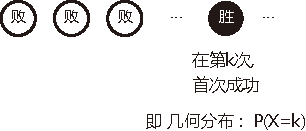
\includegraphics[width=0.4	\textwidth]{/0146.pdf} \\
	
	
	
	所以, 只要看到``首次发生"这个关键词, 我们就要想到使用``几何分布"来做. \\
	
	\begin{myEnvSample}
		射击, 命中率是0.6. \\
		则我们令 随机变量X表示``直到首次命中时, 所射击的次数" (即第一次成功时, 是第几次射击). 
		
		就有: $
		P\left( X=k \right) =\left( 1-P \right) ^{k-1}\cdot P=\left( 1-0.6 \right) ^{k-1}\cdot 0.6,\ k=1,2,3...
		$ \\
		
		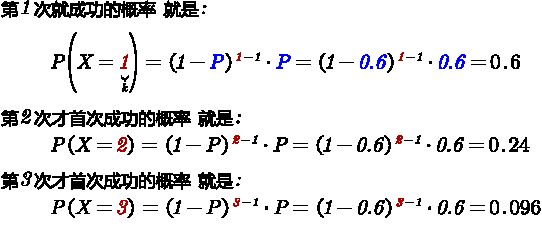
\includegraphics[width=0.7\textwidth]{/0147.pdf} \\
		
		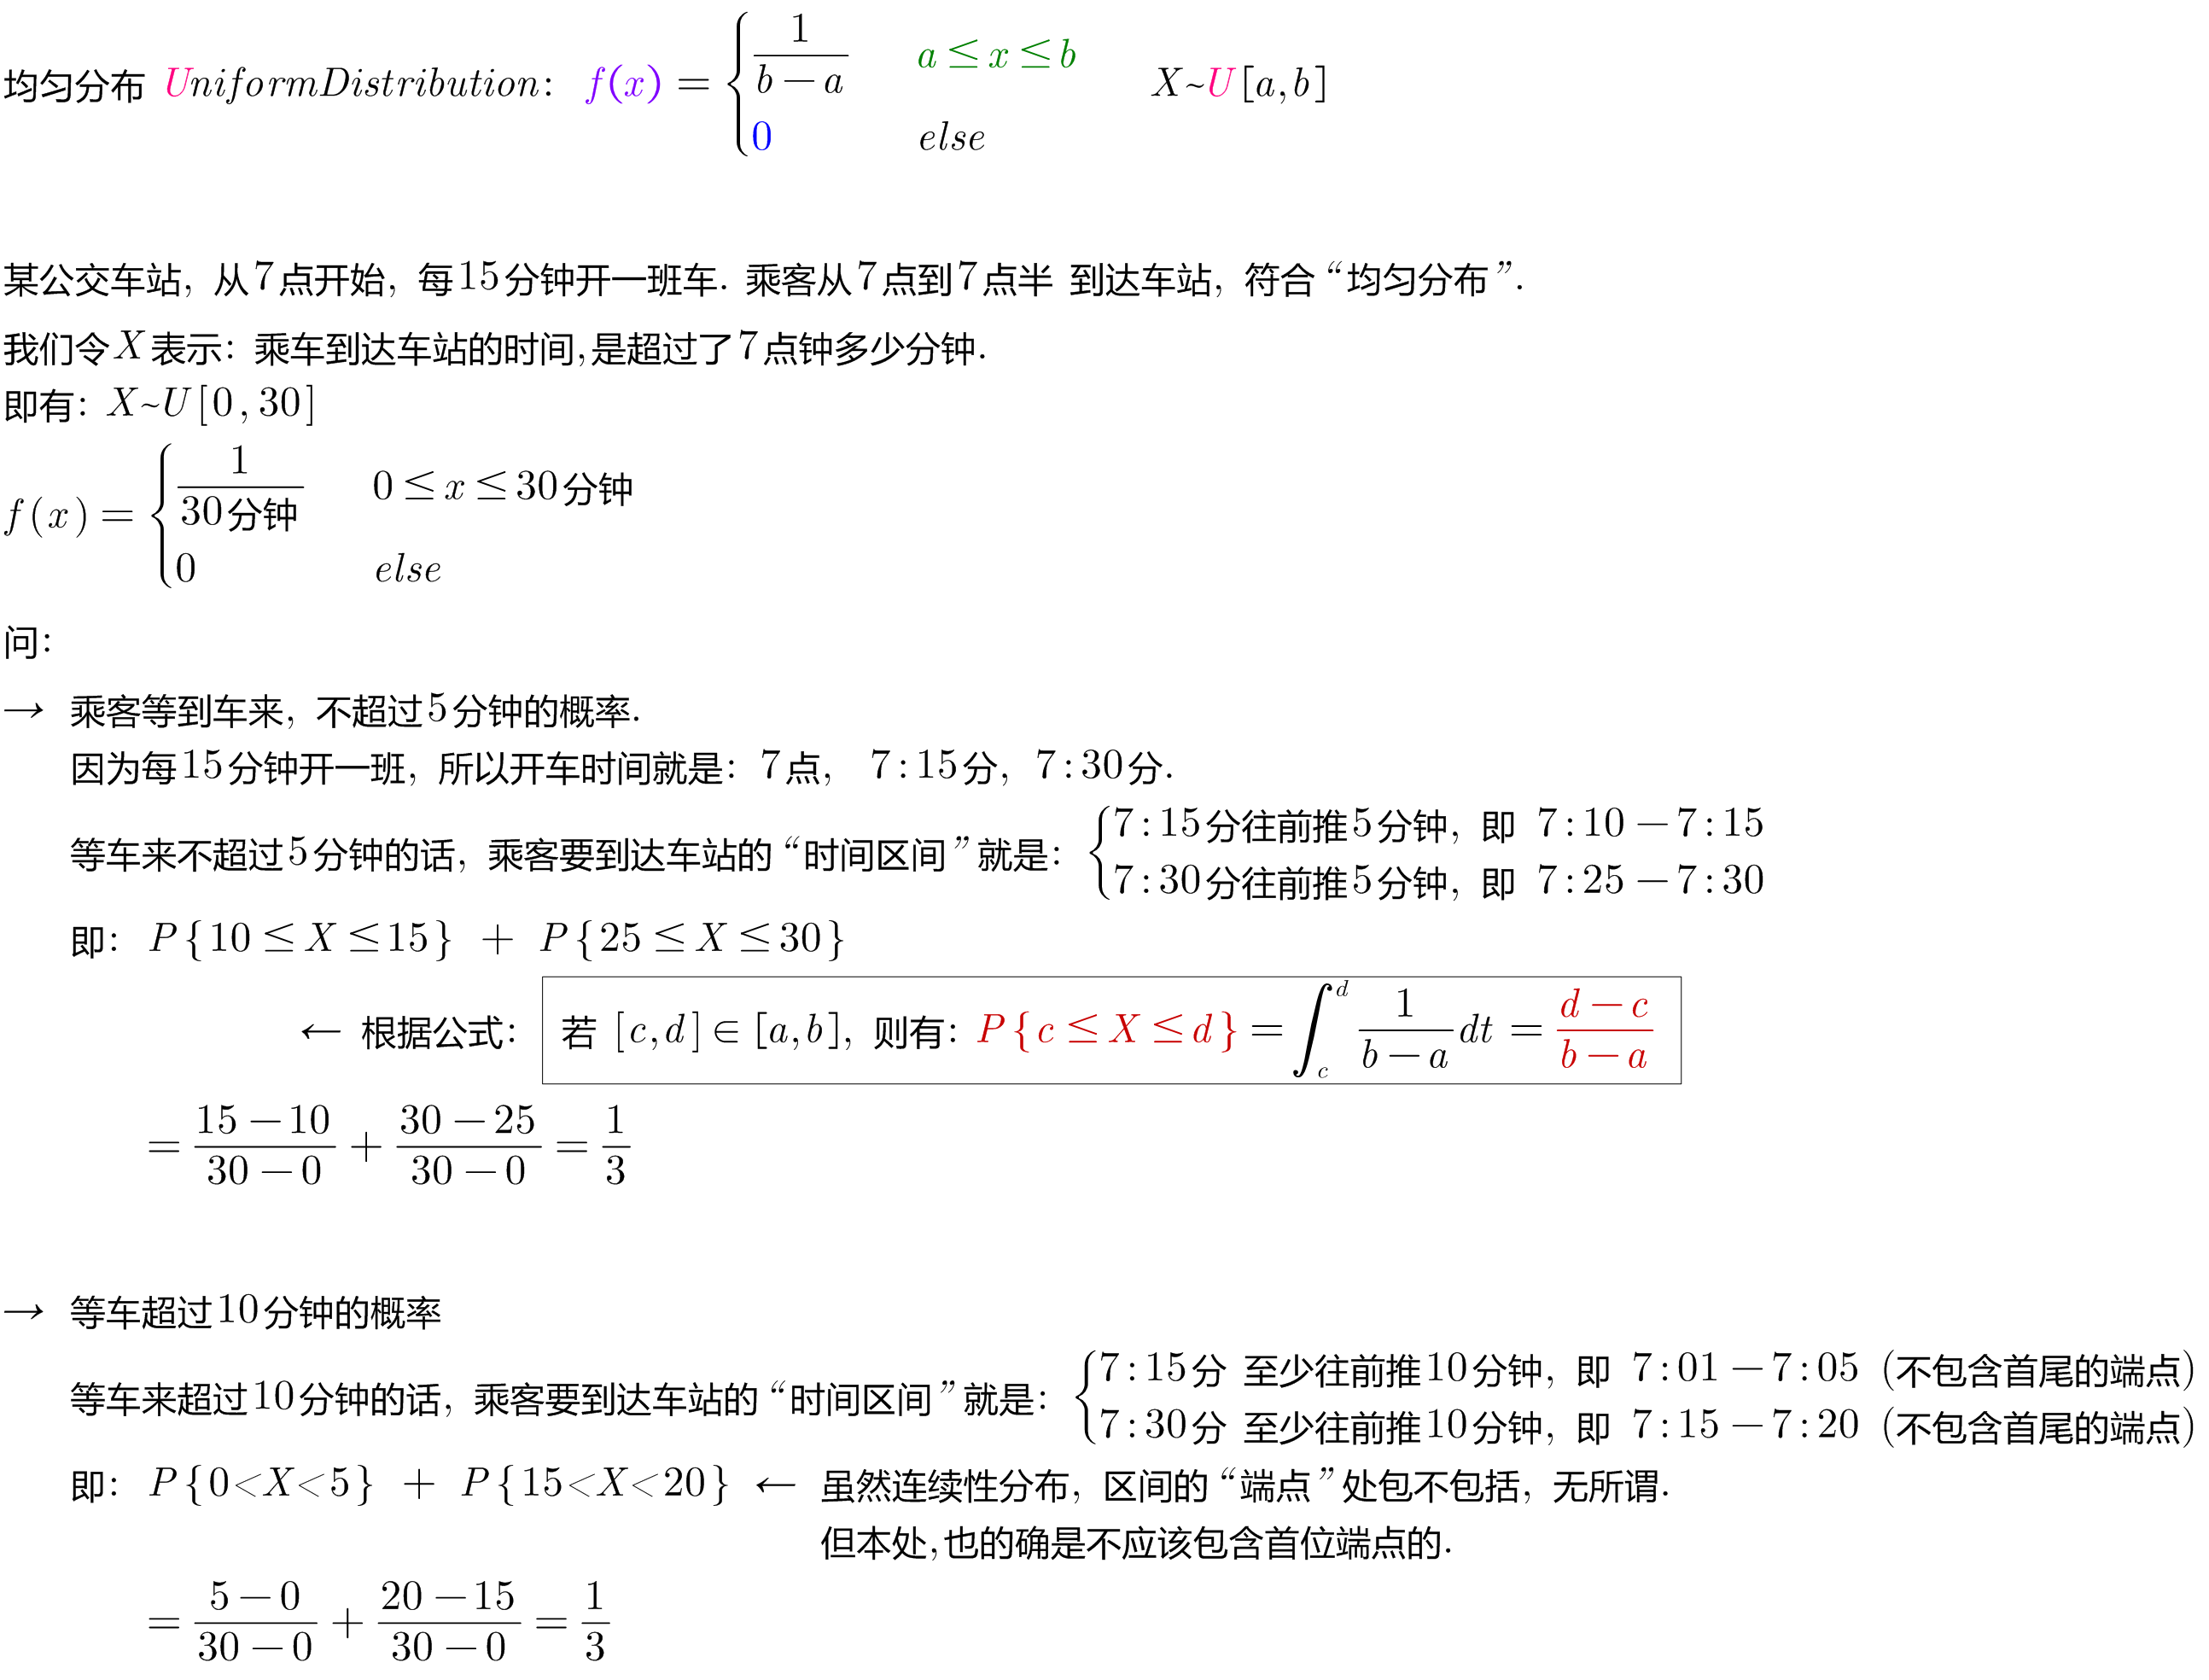
\includegraphics[width=0.9\textwidth]{/0148.png} \\
	\end{myEnvSample}
	
	
	
	
	几何分布 Geometric distribution 是``离散型数据"的概率分布. \\
	``几何分布"是``帕斯卡分布"当 r=1 时的特例. \\
	 (帕斯卡分布 Pascal distribution 是: 进行多次重复、独立的伯努利试验, 直到出现r次某事件成功为止. 即: 随机变量X表示所需的试验次数. 用 P(X=k)来表示``帕斯卡分布". 即: $P\left( X=k \right) =C_{k-1}^{r-1}\cdot P^r\cdot \left( 1-P \right) ^{k-r},\ \ k=r,r+1,...$) \\
	
	
	
	
	
	
	
	
\end{document}